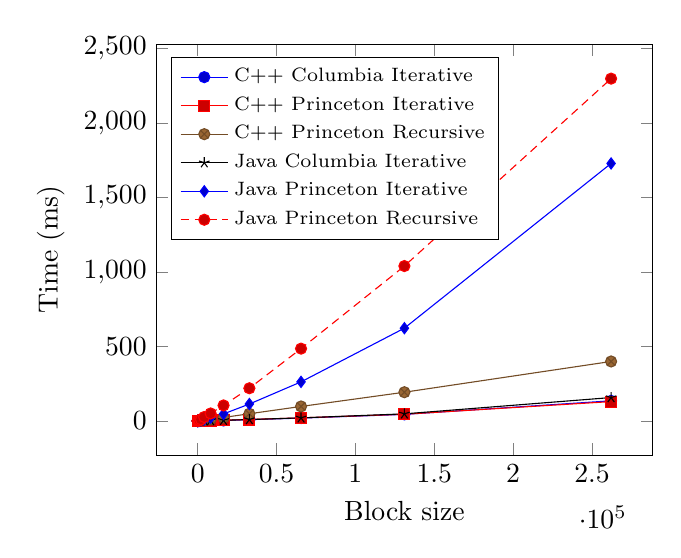
\begin{tikzpicture}
\begin{axis}[xlabel={Block size},ylabel={Time (ms)},width=0.65\linewidth,legend pos=north west,scaled y ticks = false,legend cell align=left,legend style={font=\scriptsize}]
\addplot coordinates {
(16, 0.0049)
(32, 0.0051)
(64, 0.0052)
(128, 0.0071)
(256, 0.0160)
(512, 0.0223)
(1024, 0.0516)
(2048, 0.1206)
(4096, 0.8794)
(8192, 1.8030)
(16384, 2.9629)
(32768, 8.2847)
(65536, 18.8158)
(131072, 43.7807)
(262144, 134.8093)
};
\addplot coordinates {
(16, 0.0090)
(32, 0.0128)
(64, 0.0188)
(128, 0.0292)
(256, 0.0541)
(512, 0.1038)
(1024, 0.2082)
(2048, 0.4536)
(4096, 0.9690)
(8192, 2.0605)
(16384, 4.5027)
(32768, 9.6797)
(65536, 20.3049)
(131072, 44.5770)
(262144, 129.5150)
};
\addplot coordinates {
(16, 0.0215)
(32, 0.0328)
(64, 0.0617)
(128, 0.1252)
(256, 0.2642)
(512, 0.5573)
(1024, 1.1380)
(2048, 2.4265)
(4096, 5.1699)
(8192, 10.7496)
(16384, 22.8640)
(32768, 48.0022)
(65536, 96.9572)
(131072, 192.4607)
(262144, 398.9698)
};
\addplot coordinates {
(16, 0.0265)
(32, 0.0658)
(64, 0.0179)
(128, 0.0158)
(256, 0.0290)
(512, 0.0603)
(1024, 0.1289)
(2048, 0.3302)
(4096, 0.8200)
(8192, 2.1766)
(16384, 3.9995)
(32768, 8.9846)
(65536, 20.2833)
(131072, 47.2950)
(262144, 156.7135)
};
\addplot coordinates {
(16, 0.1398)
(32, 0.0492)
(64, 0.1078)
(128, 0.1991)
(256, 0.3547)
(512, 0.7740)
(1024, 1.7228)
(2048, 3.8546)
(4096, 8.8053)
(8192, 21.1757)
(16384, 46.8150)
(32768, 113.1953)
(65536, 261.9954)
(131072, 622.4328)
(262144, 1728.4640)
};
\addplot coordinates {
(16, 0.0387)
(32, 0.0850)
(64, 0.1761)
(128, 0.4199)
(256, 0.8938)
(512, 1.9155)
(1024, 4.1350)
(2048, 9.2740)
(4096, 26.0912)
(8192, 50.0776)
(16384, 103.9682)
(32768, 219.0208)
(65536, 485.1020)
(131072, 1039.4937)
(262144, 2297.8011)
};
\legend{C++ Columbia Iterative,C++ Princeton Iterative,C++ Princeton Recursive,Java Columbia Iterative,Java Princeton Iterative,Java Princeton Recursive}
\end{axis}
\end{tikzpicture}
